\begin{figure}
  \centering
  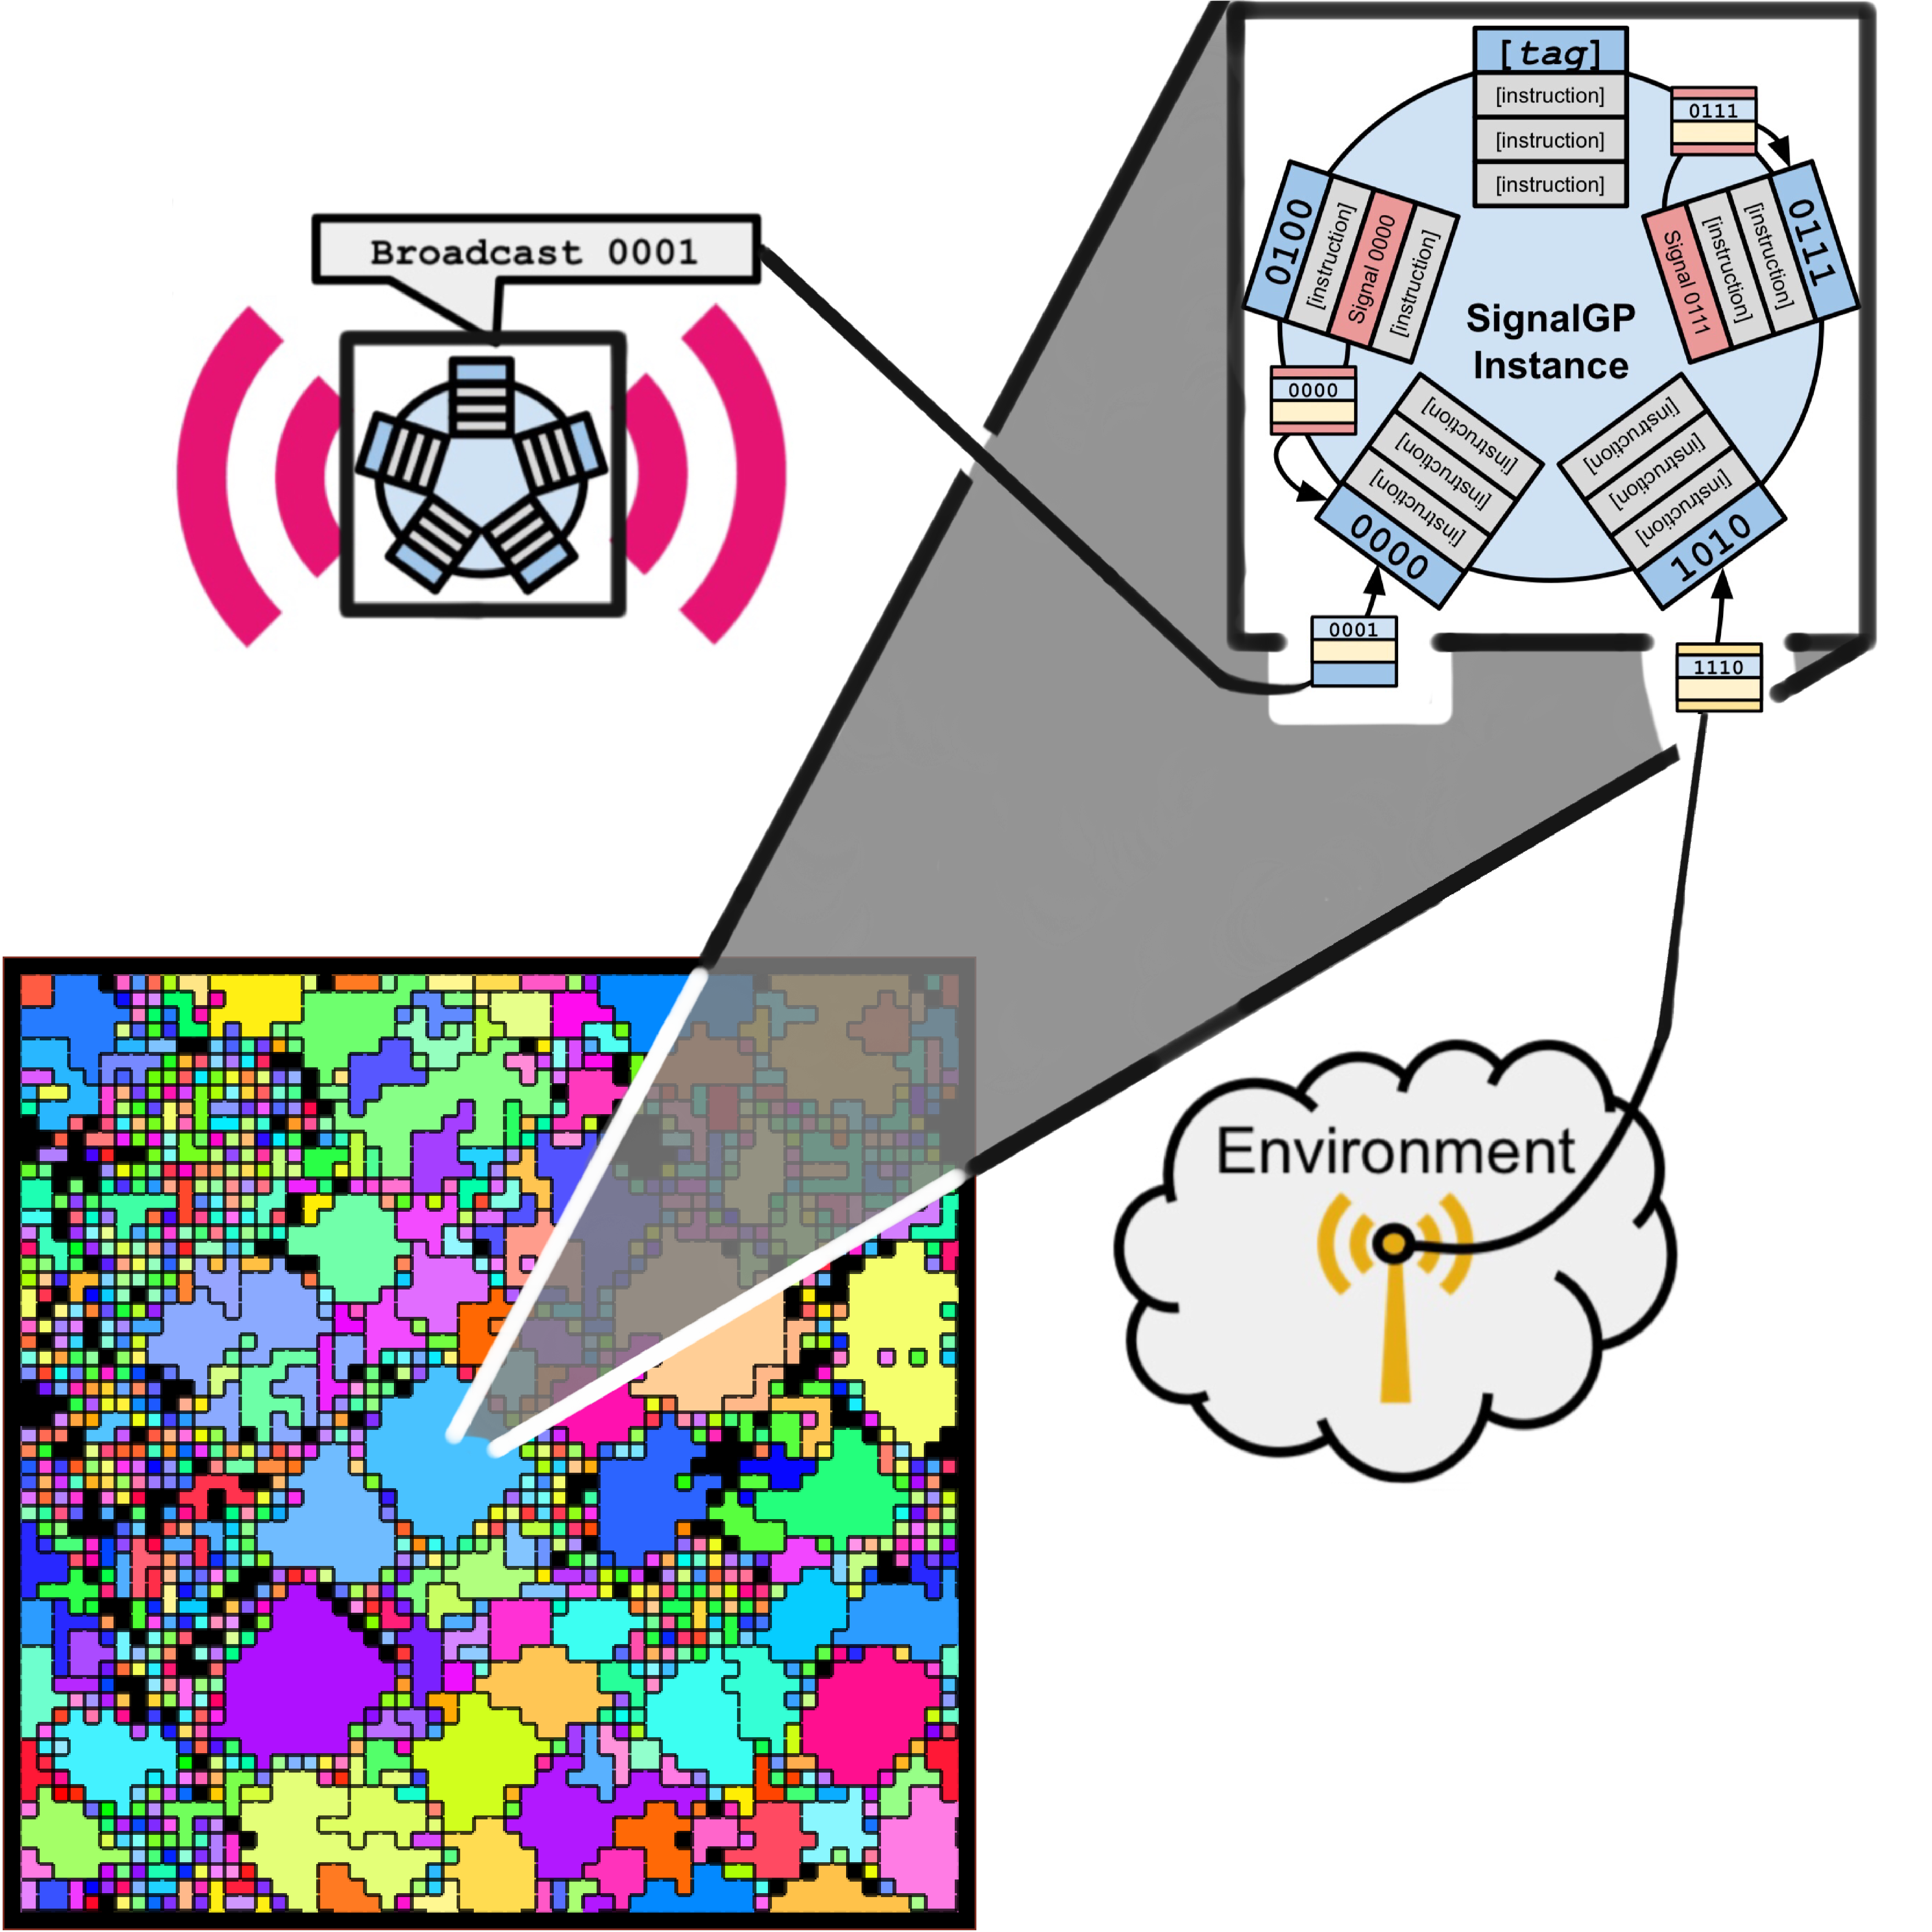
\includegraphics[width=\textwidth]{img/schematic}
  \vspace{-10ex}
  \begin{columns}
  \begin{column}{0.52\textwidth}
  \end{column}
  \begin{column}{0.48\textwidth}
  \caption{
  Experiments track digital cells on a fixed-size toroidal grid (bottom left).
  The size of a cell's resource-collecting group (contiguous same-color clumps) determines cellular reproduction rate.
  Per-cell resource-collection rate increases with group size up to a threshold group size, where it begins to diminish.
  Heritable SignalGP programs (inset, top right) \cite{Lalejini2018-GECCO} govern each cell, controlling when to reproduce, where to place the daughter cell, whether the daughter cell should grow the parent's group or start a new group, apoptosis, resource sharing, and intercellular communication.
  }
  \label{fig:model}
  \end{column}
  \end{columns}
\end{figure}
